%---------------------------------------------------------------------------------------------
%	INITIAL DOCUMENT CONFIGURATIONS
%---------------------------------------------------------------------------------------------
\documentclass[12pt, oneside, openany, a4paper, english, brazil]{abntex2}

\usepackage{cmap}				
\usepackage{lmodern}			
\usepackage[T1]{fontenc}
\usepackage[utf8]{inputenc}		
\usepackage{indentfirst}		
\usepackage{color}				
\usepackage{graphicx}			
\usepackage{multicol}
\usepackage{multirow}
\usepackage{lipsum}			
\usepackage[brazilian,hyperpageref]{backref}
\usepackage[alf]{abntex2cite}	
\usepackage{subfig} 
\usepackage{titlesec}

\titleformat{\section}{\Large\scshape\raggedright}{}{0em}{}[\titlerule] 
\titlespacing{\section}{0pt}{3pt}{3pt} 

%---------------------------------------------------------------------------------------------
% INIT DOCUMENT
%---------------------------------------------------------------------------------------------

\begin{document}

% Removes page numbering
\pagestyle{empty} 

%---------------------------------------------------------------------------------------------
%	NAME AND CONTACT INFORMATION
%---------------------------------------------------------------------------------------------

\par{
	\raggedright{\Huge Marcos Vinicius Ribeiro Silva   }
	\raggedleft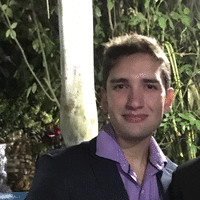
\includegraphics[scale=0.3]{Pictures/Me}
\par}

\section{Dados pessoais}

\begin{tabular}{rl}
	\textsc{Data de Nascimento:} & 06/11/1992\\
	\textsc{Celular:} & (62) 9 8156-1292\\
	\textsc{Email:} & \href{mailto:marcos.v.silva@live.com}{marcos.v.silva@live.com} \\
	\textsc{GitHub:} & \href{https://github.com/marcosvsilva}{marcosvsilva} \\
	\textsc{Lattes:} & \href{ http://lattes.cnpq.br/6930019751033452}{Marcos Vinicius} \\
	\textsc{Objetivo:} & Engenharia de Software e Ciências de Dados \\
\end{tabular}

%---------------------------------------------------------------------------------------------
%	WORK EXPERIENCE 
%---------------------------------------------------------------------------------------------

\section{Formação Acadêmica}

\begin{tabular}{p{2.2cm}|p{12cm}}
    \emph{Mestrado}
    & \emph{em Ciências da Computação} \\
    & \emph{Instituto de Informática da Universidade Federal de Goiás} \\
    & \emph{Aluno especial de Mineração de Dados; Redes Neurais Profundas} \\
    & Período: 1º semestre de 2018 \\
\end{tabular}

\begin{tabular}{p{2.2cm}|p{12cm}}
    \emph{Graduação}
    & \emph{em Engenharia de Software} \\
    & \emph{Instituto de Informática da Universidade Federal de Goiás} \\
    & Término: 2018\\
\end{tabular}

\begin{tabular}{p{2.2cm}|p{12cm}}
    \emph{Graduação}
    & \emph{em Ciências da Computação}\\
    & \emph{Instituto de Informática} da \emph{Universidade Federal de Goiás} \\
    & Ano da Interrupção: 2014\\
\end{tabular}

%---------------------------------------------------------------------------------------------
%	EDUCATION
%---------------------------------------------------------------------------------------------

\section{Experiência Profissionais e Desenvolvimento}

\begin{tabular}{p{3.5cm}p{11cm}}
    \textsc{Novembro 2017} - & Desenvolvedor de Software \\
    \textsc{Atual} & Siagri Sistemas de Gestão LTDA \\
    \textsc{} & Desenvolvimento de novas funcionalidades e aplicações em linguagem Delphi para ERP de gestão de agribusiness, trabalho de relacionamento do escopo e entregas contínuas do scrum, correção de falhas imediatas e manutenção corretiva e preventiva de sistemas, implementação de camada de persistência de dados em linguagem PL-SQL utilizando banco de dados relacional Oracle e Firebird
\end{tabular}

\begin{tabular}{p{3.5cm}p{11cm}}
    \textsc{Março 2017} - & Desenvolvedor de Software \\
    \textsc{Setembro 2017} & SIACON Consultoria em Software LTDA ME \\ 
    \textsc{} & Solução de bugs e falhas, análise e implementação de melhorias, estruturação modelagem e criação de serviços, ferramentas e relatórios em linguagem Delphi e \texttt{C\#}, manutenção e aprimoramento da camada de persistência em linguagem SQL
\end{tabular}                                    

\begin{tabular}{p{3.5cm}p{11cm}}
    \textsc{Abril 2013} - & Projeto de extensão \\
    \textsc{Outubro 2015} & Universidade Federal de Goiás \\
    \textsc{} & Programa de Treinamento para a Olimpíada Brasileira de Informática Cargo: Professor titular do treinamento para a Olimpíada Brasileira de Informática dedicada a estudantes do ensino fundamental e médio, com base em fundamentos básicos da programação de computadores na linguagem C e C++
\end{tabular}

\begin{tabular}{p{3.5cm}p{11cm}}
    \textsc{Setembro 2013} - & Desenvolvedor Delphi \\
    \textsc{Setembro 2016} & Jave Informática LTDA \\ 
    \textsc{} & Manutenção e inovação de plataformas em Linguagem Delphi com utilização de componentes próprios e de terceiros com conexão direta e indireta a banco de dados relacionais utilizando linguagem SQL
\end{tabular}

%---------------------------------------------------------------------------------------------
%	COMPUTER SKILLS 
%---------------------------------------------------------------------------------------------

\section{Qualificações}

\begin{tabular}{p{5.5cm}p{9cm}}
    \textsc{Inteligência Artificial:} & Machining Learning, Data Mining, Data Science, Big Data \\
    \textsc{Conhecimento:} & Delphi, Python, C, C++, PL-SQL, \texttt{C\#}, Java, Android, \LaTeX \\
    \textsc{Banco de Dados:} & Oracle, SQL Server, MySQL, SQLite, PostgreSQL, MongoDB, Firbird \\
    \textsc{Ambiente Integrado:} & CodeGear RAD Studio, IntelliJ IDEA, PyCharm, Jupyter Notebook, Android Studio, SQL Server Management Studio, Eclipse, Visual Studio \\
    \textsc{Design Patterns:} & Factory Method, Iterator \\
\end{tabular}

%---------------------------------------------------------------------------------------------
%	SCHOLARSHIPS AND ADDITIONAL INFO
%---------------------------------------------------------------------------------------------

\section{Atividades complementares}

\begin{tabular}{rl}
    2011 & Sociedade Brasileira para o Progresso da Ciência. 2011 \\
    2014 & Google Developers Group (GDG) DevFest Goiânia. 2014 \\
\end{tabular}

%---------------------------------------------------------------------------------------------
% CLOSED DOCUMENT
%---------------------------------------------------------------------------------------------

\end{document}